\section{The Platform}
\label{sec:platform}

\subsection{Overview: One Loop, Four Modules, Two Screens}
\label{sec:platform-overview}

The platform decomposes the adaptive reading loop into four concerns chosen along the axis of replaceability: \emph{sensing} produces a continuous stream of gaze samples; \emph{analysis} projects that stream into oculomotor events (fixations, saccades, regressions); \emph{decision} consumes the analysed state and returns at most a proposal to intervene; and \emph{intervention} validates a proposal and commits a change to the text at a controlled boundary.
Each concern sits behind a stable contract with a uniform shape: a module is identified by a stable provider identity and exposes a single operation that receives an immutable snapshot of the relevant session state and returns an optional result.
Because a module is handed a copy of what it needs rather than a reference to live state, it can neither reach into nor mutate the core; and because the runtime resolves modules from a per-concern registry by identifier, never naming a concrete implementation, adding a module is one registration and no existing code changes.
The backend (\,.NET\,) owns all authoritative session state; the dependency rule that the core references no infrastructure is enforced by the build itself, so a violation is a compile error rather than a convention.

Two browser surfaces of a single web frontend face the two people in the room (Figure~\ref{fig:screens}).
The participant surface renders the reading material as reflowable, tokenised text.
The researcher console mirrors the same text and overlays the participant's live gaze, a fixation heat map, and recent saccades, so the researcher sees not merely where the participant looks but how they read.
The surfaces never communicate with each other; both render the same backend-owned snapshot, so they cannot disagree.
Discrete commands (configure a session, change an intervention policy, start, stop) travel over a request-and-response channel, while the high-frequency gaze stream travels over a separate realtime channel (a single WebSocket per client), a split that keeps the per-sample path free of the locking that guards session lifecycle.
Figure~\ref{fig:loop} traces one cycle of the loop across these parts.

\begin{figure}
  \centering
  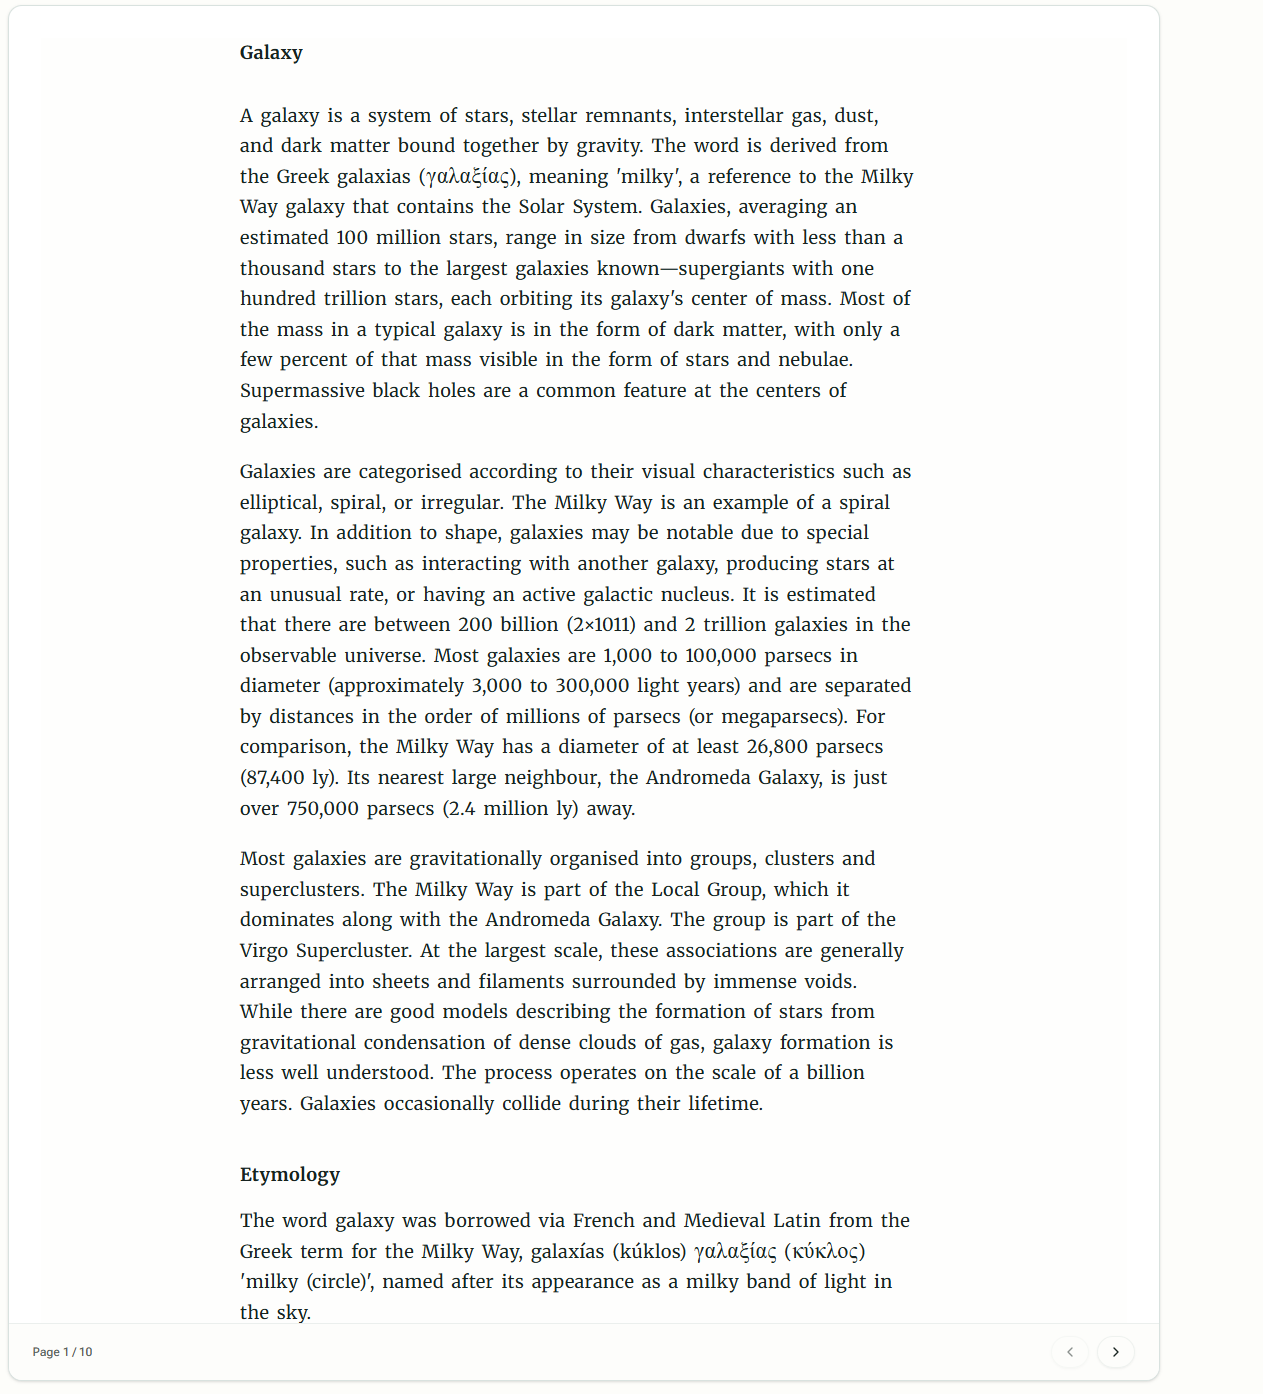
\includegraphics[width=0.49\columnwidth]{figures/ReadingView.png}\hfill
  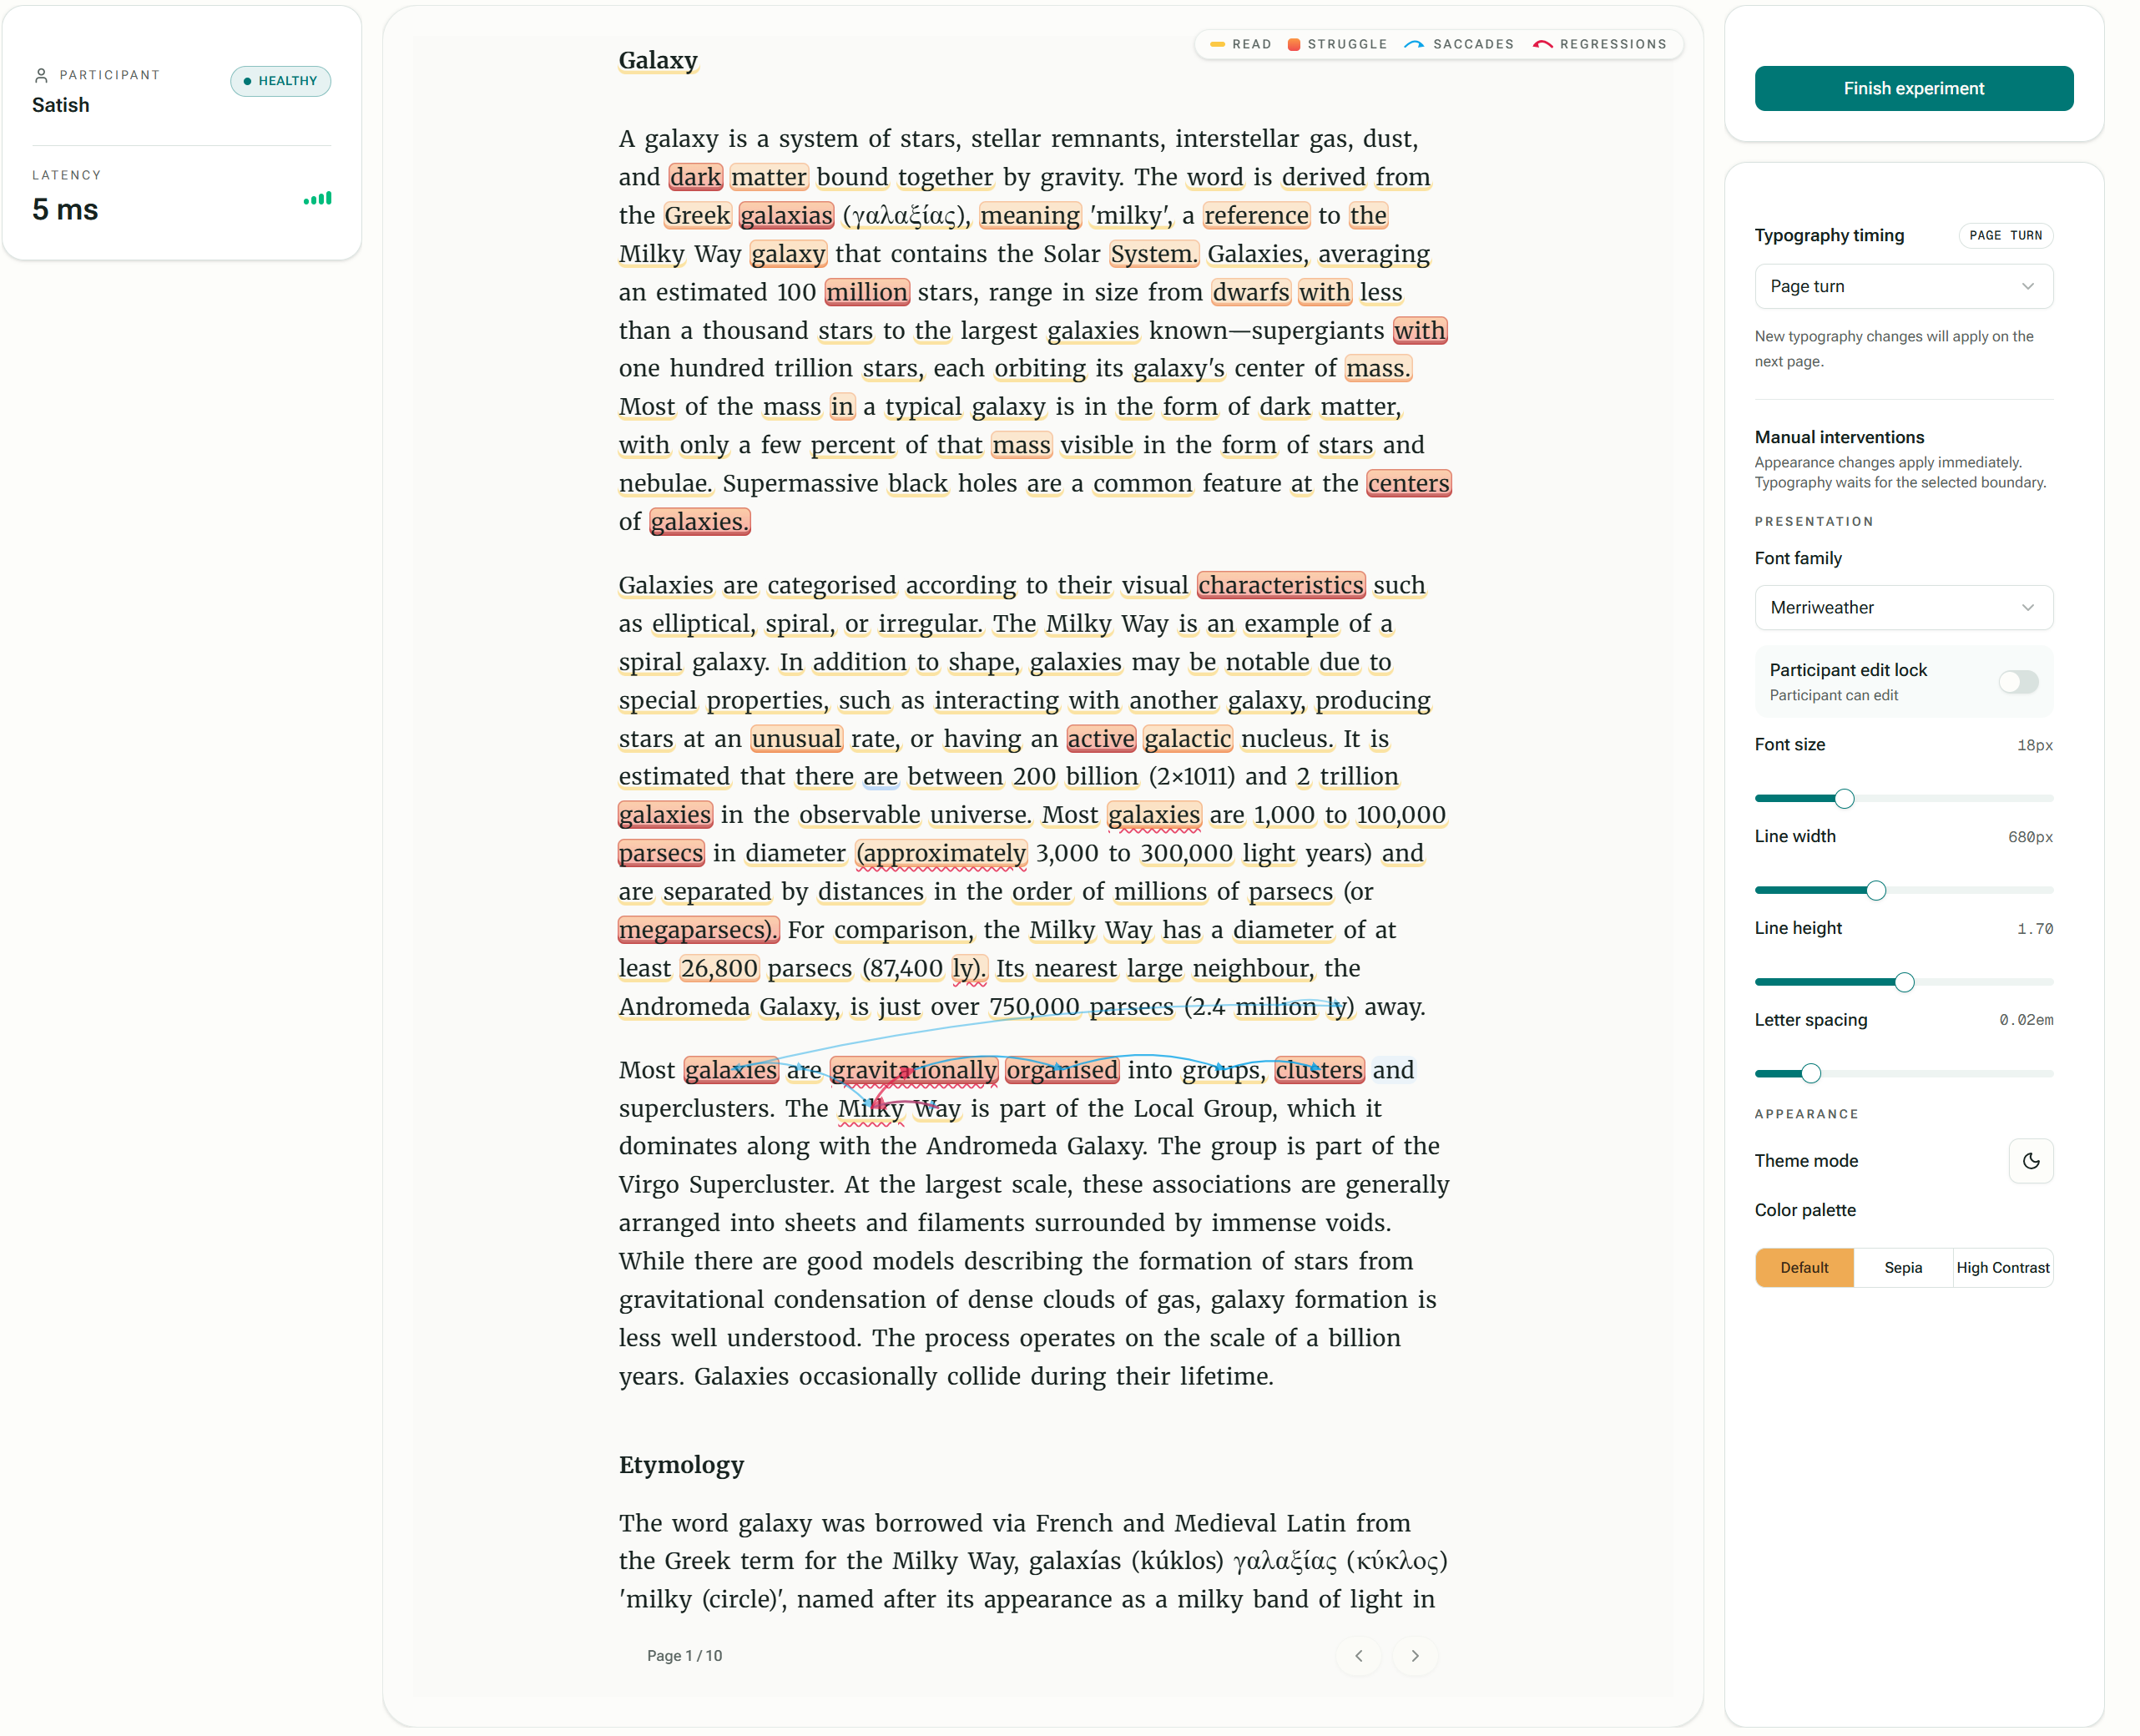
\includegraphics[width=0.49\columnwidth]{figures/ResearcherLiveView.png}
  \caption{The two operated surfaces: the participant reader (left) and the researcher console mirroring the same text with live gaze, fixation, and saccade overlays and the intervention controls (right).}
  \Description{Two application screenshots side by side. The left shows a clean reading view with a paragraph of text. The right shows the same text overlaid with gaze markers and, beside it, control panels for interventions and session state.}
  \label{fig:screens}
\end{figure}

\begin{figure*}
  \centering
  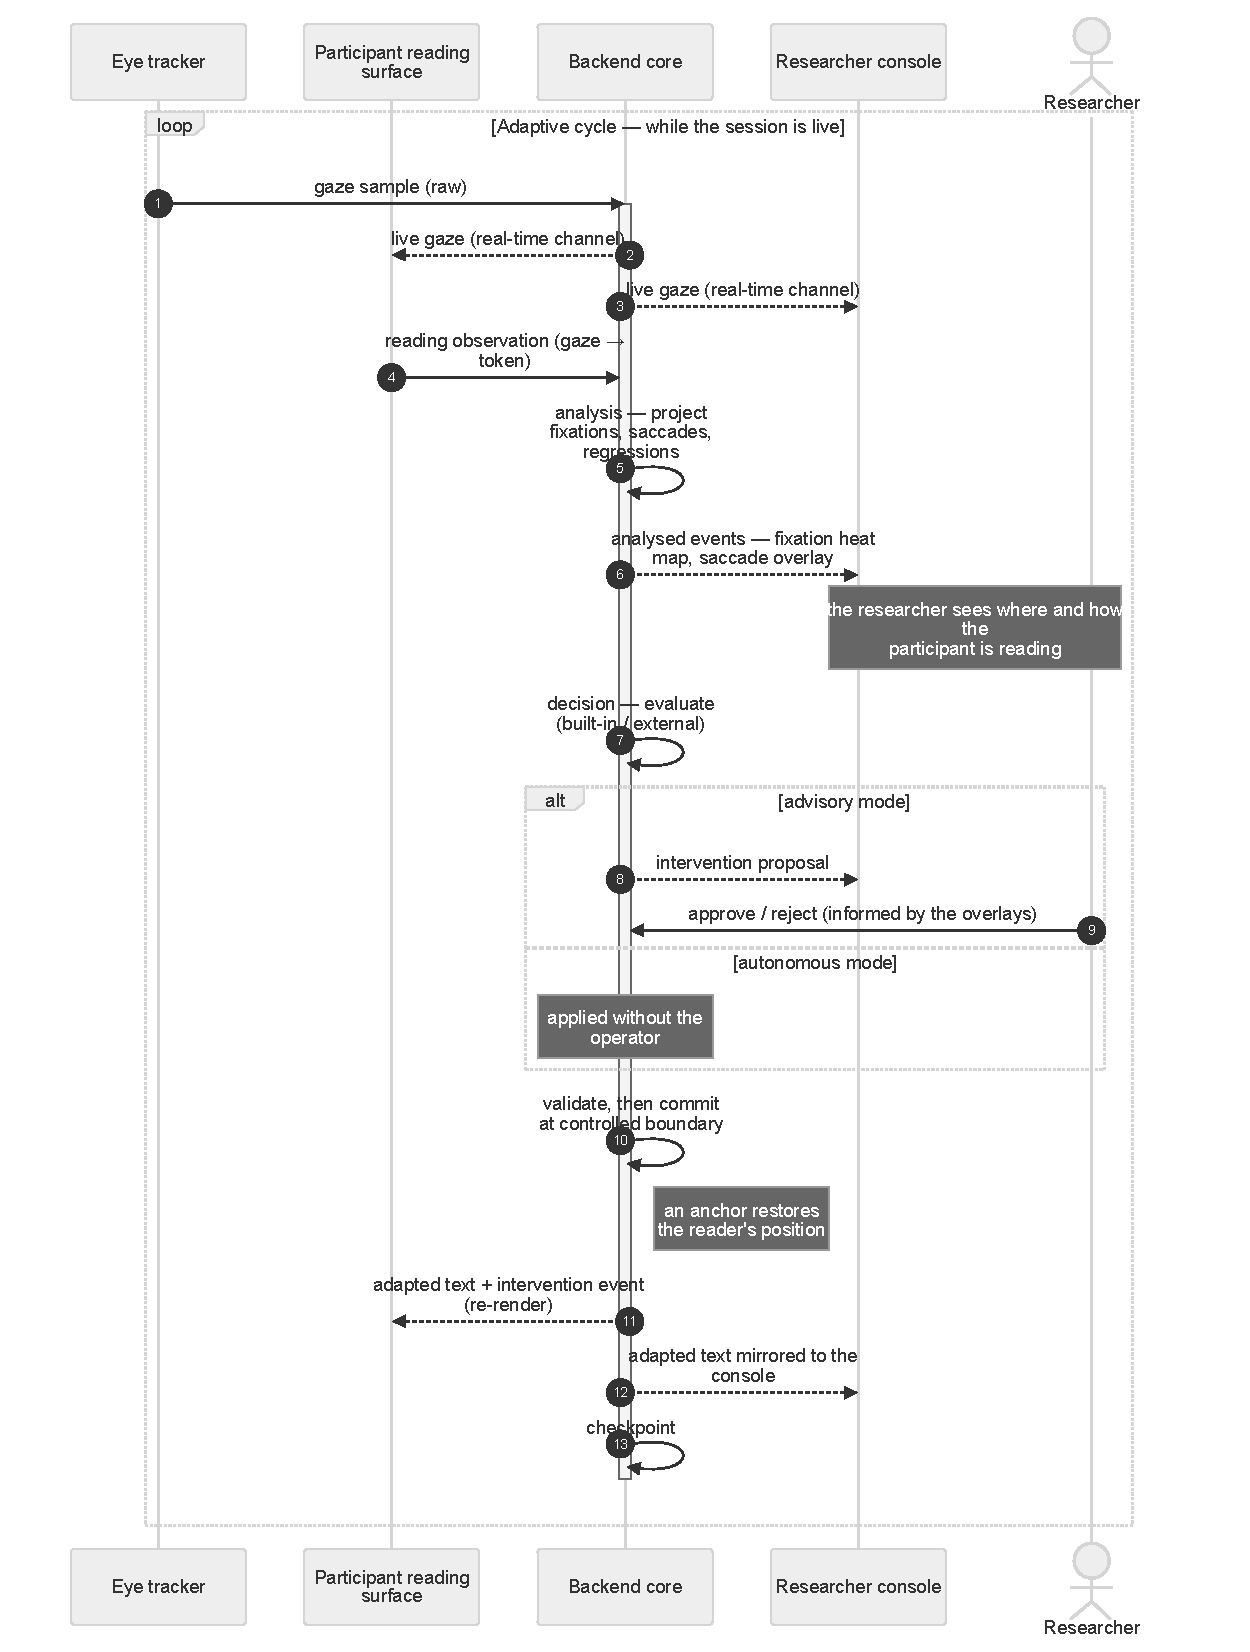
\includegraphics[width=0.92\textwidth]{figures/adaptive-loop.pdf}
  \caption{One iteration of the real-time adaptive loop.
  A gaze sample is mirrored to both surfaces over the realtime channel; the participant surface, which alone knows the rendered layout, maps it to a token and returns an enriched observation; analysis projects observations into oculomotor events; a decision (built-in, external, or the researcher acting manually) yields at most one proposal, which in advisory mode waits for researcher approval; the intervention commits at a controlled boundary and the adapted text returns to both surfaces.
  Persistence checkpoints are written best-effort throughout.}
  \Description{A sequence diagram showing messages between the participant surface, the backend core with its analysis, decision, and intervention stages, the researcher console, and a persistence store, forming one cycle from gaze sample to committed intervention.}
  \label{fig:loop}
\end{figure*}

\subsection{Sensing and Gaze-to-Word Mapping}
\label{sec:platform-mapping}

Sensing is a port with interchangeable sources.
The primary adapter subscribes to a Tobii eye tracker's native callback and republishes each sample (per-eye position on the display area normalised to the unit square, pupil data, validity flags, device timestamp) into the domain; a simulated source emits samples of exactly the same shape from the mouse cursor, so the full loop runs with or without hardware and the downstream stages cannot tell which source produced a sample.
On the backend, the gaze path is deliberately lock-free: each arriving sample is sanitised, published with a volatile write as the latest value, counted atomically, and broadcast, without acquiring the lock that serialises lifecycle commands.
The heavier modular pipeline of analysis, decision, and intervention runs at the cadence of analysed-state changes rather than once per raw sample, which keeps the indirection introduced for modularity off the per-sample path.
On the participant surface, snapshot bursts are coalesced to a single React commit per animation frame, so the live view re-renders at display rate regardless of the inbound message rate while never dropping the newest state.

The spatial half of the pipeline runs in the reader, the only place the rendered layout exists.
Every word is a tokenised span whose on-screen box is measured from the live DOM and re-measured whenever the layout changes, prompted by mutation, resize, and scroll observers.
An incoming gaze point is smoothed adaptively, mapped into the reading area, and hit-tested in two stages: first the line, scored by vertical distance with a fixed hysteresis bonus for the line currently being read, so that vertical jitter of the order of the line spacing does not flicker attribution between neighbours; then the nearest word on that line.
The mapping has two properties that matter for an adaptive reader.
It is resolution-independent, because the tracker reports gaze as a fraction of the display and the words are measured live rather than assumed.
And it is reflow-proof by construction: a typographic intervention that moves every word to a new position cannot invalidate the mapping, because the next sample is hit-tested against the boxes as they now are, which is precisely the failure mode a coordinate-based scheme would suffer.
The result of the stage is a token-level reading observation (token, line, and block identity) published back to the backend.

\subsection{Eye-Movement Analysis as a Replaceable Strategy}
\label{sec:platform-analysis}

The temporal half of the pipeline is an explicit analysis strategy behind its own contract.
The built-in strategy realises the area-of-interest branch of the classical taxonomy \cite{salvucci2000identifying}: since each observation is already bound to a word, the word itself is the area of interest, and a fixation is confirmed from accumulated dwell, with thresholds of 90\,ms initially, 70\,ms for a candidate on the same line, and 135\,ms across a line change, the latter raised because cross-line movement is larger and noisier.
For per-word attention statistics, dwell below 45\,ms is discarded as noise and dwell of at least 130\,ms counts as a fixation, with the band between recorded as a skim, so the statistics separate words that were read from words the gaze merely crossed.
Saccades are classified from token and line deltas, and a backward or line-change-backward saccade is counted as a regression, the standard oculomotor sign of reading disruption \cite{rayner1998eyemovements}.
The strategy is a pure function of the observation and the prior state, so replaying the same observations yields the same events, and it is resolved from a registry, so an external analysis provider can replace it at runtime (Section~\ref{sec:platform-decision}).

\subsection{The Decision Boundary and Execution Modes}
\label{sec:platform-decision}

Decisions about when and how to adapt the text can come from three sources: the researcher acting manually from the console, a built-in rule-based strategy, or an external provider.
Two execution modes cover the supervision spectrum without structural change: in \emph{advisory} mode every machine proposal is surfaced on the console and applied only when the researcher approves it, and in \emph{autonomous} mode a permitted proposal is applied directly.
Every proposal passes through an explicit lifecycle with exactly one terminal outcome (approved, rejected, applied, or superseded when a newer proposal or a mode change overtakes it), so the text never adapts on a decision that no longer holds, and every outcome is logged.

External providers connect out of process over a documented WebSocket protocol: a handshake in which the provider declares its identity, modules, and capabilities and receives an accept-or-reject reply, followed by heartbeats and tunnelled traffic.
What crosses the boundary is a fixed vocabulary: outward, an immutable session snapshot and the stream of analysed signals (reading focus, attention summary, oculomotor events); inward, a proposal pairing an observed signal and a short human-readable rationale with the identity of an intervention module and the parameters to apply.
The seam commits the platform to signals in and a proposal out, but not to any particular way of arriving at the proposal, which is what makes an AI-driven provider a configuration rather than a rewrite.
An external decision is applied through exactly the same validation and logging path as a built-in one, and a provider that stops sending heartbeats or disconnects is dropped, with the affected concern degrading to its built-in fallback and the transition recorded in the session log.
The same provider framework serves the analysis seam in the same way, one mechanism for two concerns.

\subsection{Context-Preserving Interventions}
\label{sec:platform-context}

Typographic interventions are the platform's actuator: built-in modules cover font family, font size, line width, line height, letter spacing, theme, and palette.
Appearance-only changes commit immediately.
Layout-changing interventions instead wait for a chosen commit boundary (immediately, at the end of the sentence or paragraph being read, or at the page turn), so a reflow lands at a natural break rather than mid-line.

Around the commit, the reader runs a capture-and-restore mechanism.
An anchor is captured continuously (every 120\,ms and on content changes), preferring the word the participant is currently reading, degrading to a visible fallback word or its enclosing block, and recording the element's identity together with its viewport offset; anchors older than 15\,s are rejected as stale.
When a layout change commits, the reader re-locates the anchor in the reflowed document (degrading sentence to token to block) and scrolls it back to the viewport offset it held before the change.
The residual error between target and achieved offset is then measured, graded (preserved, degraded, or failed, with tolerances of 72\,px for a full reflow and 48\,px to 120\,px otherwise), and written into the session record next to the intervention that caused it.
Optionally, the restored sentence is briefly highlighted and fades over about three seconds, drawing the eye back to the resume point, which corresponds to the highlighting component that prior work found effective for recovery \cite{jensen2025context}.

This restore-to-captured-offset design is itself a product of the platform's self-measurement.
Our original strategy re-established the committed sentence near the top of the reading area; Section~\ref{sec:eval-context} shows how the recorded outcomes exposed that this over-repositioned the reader on small reflows, and how the revision removes the defect.
Because every intervention's graded outcome and residual are in the record, a later analysis can ask not only whether an intervention helped a reader but what it cost them in lost position.

\subsection{Researcher Console, Session Record, and Replay}
\label{sec:platform-record}

A session is operated end to end from the researcher console.
Setup is a gated stepper: a session cannot start until a participant is saved, a licensed eye tracker is selected, a calibration has passed validation, and reading material is chosen, with the gates re-checked by the backend at the moment of start.
Calibration uses 9-, 13-, or 16-point presets followed by a five-target validation that computes angular accuracy and precision, passing only when the averages stay within fixed bounds and at least four fifths of the points pass.
During the run, the console shows the mirror with live analysis overlays, the current gaze-validity rate, and the measured client latency, and carries the intervention and typography controls together with the approval queue in advisory mode.

Everything that happens flows into one authoritative, schema-versioned session record owned by the backend: the run parameters and presentation baseline, calibration metrics, screen geometry, the raw gaze stream, derived oculomotor events, decision proposals and their outcomes, interventions and their context-preservation outcomes, and quiz responses, each entry stamped with a monotonic sequence number and timestamp.
The record is not assembled after the fact; it is the same structure a background worker checkpoints throughout the session, so durability and export are one artifact and an interrupted session is recoverable from its latest checkpoint.
A completed record exports to JSON and CSV, re-imports through a version-gated schema check, and replays in the reading interface with scrubbing, variable speed, and jump-to-event navigation.
Replay is the operational definition of the record's completeness: if a session can be re-presented and re-analysed from the record alone, the record contains what reproducibility requires.
The platform also emits a telemetry record (round-trip times per client, achieved sampling rate, validity, and decision-path latencies) against an explicit 100\,ms budget, which is the instrumentation behind Section~\ref{sec:eval-perf}.
